\documentclass[journal, a4paper]{IEEEtran}
\usepackage{graphicx,url,amsmath, verbatim, float, moresize}   
\usepackage[brazil]{babel}
\usepackage[utf8]{inputenc, color}
\usepackage[T1]{fontenc}
\usepackage[compatibility,siunitx,  americanvoltages, americancurrents, americanresistors, europeaninductors, americanports,straightlabels, fetbodydiode, straightvoltages]{circuitikz}
\usepackage{tikz,amsmath, amssymb,bm,color,pgfkeys,siunitx,ifthen,ulem}
\usepackage{pgfplots}
\pgfplotsset{compat=1.14}
\usetikzlibrary{shapes,arrows}
\usetikzlibrary{circuits.ee.IEC}
\usetikzlibrary{arrows}
\usetikzlibrary{backgrounds,calc,positioning}
\ctikzset{tripoles/mos style/arrows}
\ctikzset{
	/tikz/circuitikz/quadpoles/coupler/width=1,%1.3
	/tikz/circuitikz/quadpoles/coupler/height=0.952,%1.3
	/tikz/circuitikz/quadpoles/coupler2/width=1,%1.3
	/tikz/circuitikz/quadpoles/coupler2/height=0.952,%1.3
	/tikz/circuitikz/quadpoles/transformer/width=1.425,%1.5
	/tikz/circuitikz/quadpoles/transformer/height=1.425,%1.5
	/tikz/circuitikz/quadpoles/transformer core/width=1.425,%1.5
	/tikz/circuitikz/quadpoles/transformer core/height=1.425,%1.5
	/tikz/circuitikz/quadpoles/gyrator/width=1.425,%1.5
	/tikz/circuitikz/quadpoles/gyrator/height=1.425,%1.5
	/tikz/circuitikz/monopoles/tlinestub/width=0.1875,%0.25 no effect!
	/tikz/circuitikz/tripoles/american and port/height=0.95,%.8
	/tikz/circuitikz/tripoles/american nand port/height=0.95,%.8
	/tikz/circuitikz/tripoles/american or port/height=0.95,%.8
	/tikz/circuitikz/tripoles/american nor port/height=0.95,%.8
	/tikz/circuitikz/tripoles/american xor port/height=0.95,%.8
	/tikz/circuitikz/tripoles/american xnor port/height=0.95,%.8
	/tikz/circuitikz/bipoles/tline/height=0.4,%0.3
%	/tikz/circuitikz/bipoles/tline/width=1.2,%0.8
	/tikz/circuitikz/bipoles/diode/height=0.375,%
	/tikz/circuitikz/bipoles/diode/width=0.375,%
	/tikz/circuitikz/bipoles/varcap/height=0.375,%
	/tikz/circuitikz/bipoles/varcap/width=0.375,%
	/tikz/circuitikz/tripoles/triac/height=1.05,%
	/tikz/circuitikz/tripoles/triac/width=0.952,%
	/tikz/circuitikz/tripoles/thyristor/height=1.05,%
	/tikz/circuitikz/tripoles/thyristor/width=0.952,%
	/tikz/circuitikz/tripoles/op amp/height=0.952,%
	/tikz/circuitikz/tripoles/op amp/width=1.2,%
	/tikz/circuitikz/tripoles/op amp/font=\footnotesize,
	/tikz/circuitikz/tripoles/gm amp/height=0.952,% 1.7
	/tikz/circuitikz/tripoles/gm amp/width=1.2,% 1.4
	%	/tikz/circuitikz/tripoles/gm amp/font=\footnotesize,
	/tikz/circuitikz/tripoles/plain amp/height=0.952,% 1.7
	/tikz/circuitikz/tripoles/plain amp/width=1.2,% 1.4
	/tikz/circuitikz/bipoles/resistor/voltage/straight label distance/.initial=.8,
	/tikz/circuitikz/bipoles/generic/voltage/straight label distance/.initial=.8,
	/tikz/circuitikz/bipoles/inductor/voltage/straight label distance/.initial=.8,
	/tikz/circuitikz/bipoles/fullgeneric/voltage/straight label distance/.initial=.8,
	/tikz/circuitikz/bipoles/capacitor/voltage/straight label distance/.initial=1.0,
	/tikz/circuitikz/bipoles/thickness=1.6,
}
\ctikzset{v/.append style={/tikz/european voltages}}

\definecolor{netlabelcolor}{rgb}{0, 0, 0.25}
\definecolor{lttotitextcolor}{rgb}{0, 0.4, 0.25}
\definecolor{lttotidrawcolor}{rgb}{0.6, 0.6, 0.6}
\definecolor{netcolor}{rgb}{0, 0, 0}

\pgfkeys{/lt2ti/netlabel/font/.initial= \small}
\pgfkeys{/lt2ti/text/font/.initial= \small}

\pgfkeys{/lt2ti/Net/.style= {netcolor}}
\tikzstyle{dashdotdotted}=[dash pattern=on 3pt off 2pt on \the\pgflinewidth off 2pt on \the\pgflinewidth off 2pt]

\pgfkeys{/lt2ti/VArrow/.style= {->,>=latex}}
\pgfkeys{/lt2ti/SArrow/.style= {->,>=angle 90}}

\begin{document}


	\title{Relatório 3 - Efeito da Realimentação Série-Paralelo em um Amplificador Transistorizado.}
	\author{Arthur Pimentel, Matheus Farias e Matheus Henrique de Araújo.

    }
	\maketitle
	\vspace{}
	
\section{Introdução}

    \tab Nesta prática, foram estudados os efeitos sofridos por um amplificador transistorizado à aplicação de duas resistências de realimentação. Procurou-se determinar a discrepância entre as resistências teóricas, simuladas e práticas. O grupo utilizou certos artifícios ferramentais, como o potenciômetro, para determinar certas medidas experimentais. Estas ferramentas serão explicadas ao longo do relatório. Procura-se verificar a validade da teoria que serviu de embasamento para esta prática.
    
\section{Análise Teórica}

    \subsubsection{Cálculos Teóricos}
    
    \tab Observa-se na Figura \ref{EM com realimentação}, o circuito de um amplificador emissor-comum com dois resistores de realimentação.
    
    \makeatletter

%% bandstop filter (adapted from highpass)
\pgfcircdeclarebipole{}{\ctikzvalof{bipoles/highpass/width}}{*bandstop}{\ctikzvalof{bipoles/highpass/width}}{\ctikzvalof{bipoles/highpass/width}}{
	\pgf@circ@res@step = \ctikzvalof{bipoles/highpass/width}\pgf@circ@Rlen
	\divide \pgf@circ@res@step by 2
	
	\pgfpathmoveto{\pgfpoint{\pgf@circ@res@left}{\pgf@circ@res@zero}}
	\pgf@circ@res@other = \pgf@circ@res@left
	\advance\pgf@circ@res@other by \pgf@circ@res@step 
	
	\ifpgf@circuit@dashed
	\pgfsetdash{{0.1cm}{0.1cm}}{0cm} 
	\fi	
	
	% draw outer box
	\pgfsetlinewidth{\pgfkeysvalueof{/tikz/circuitikz/bipoles/thickness}\pgfstartlinewidth}
	\pgfpathrectanglecorners{\pgfpoint{\pgf@circ@res@left}{\pgf@circ@res@up}}{\pgfpoint{\pgf@circ@res@right}{\pgf@circ@res@down}}
	\pgfusepath{draw}
	
	\ifpgf@circuit@inputarrow
	{
		\advance \pgf@circ@res@left by -.5\pgfkeysvalueof{/tikz/circuitikz/bipoles/thickness}\pgfstartlinewidth
		\pgftransformshift{\pgfpoint{\pgf@circ@res@left}{0pt}}
		\pgfnode{inputarrow}{tip}{}{pgf@inputarrow}{\pgfusepath{fill}}
	}
	\fi
	
	% rotate inner symbol
	\def\pgfcircmathresult{\expandafter\pgf@circ@stripdecimals\pgf@circ@direction\pgf@nil}
	\ifnum \pgfcircmathresult > 45 \ifnum \pgfcircmathresult < 135
	\pgftransformrotate{270}
	\fi\fi
	\ifnum \pgfcircmathresult > 134 \ifnum \pgfcircmathresult < 225  % 134 degree, because >= 135 is not possible
	\pgftransformrotate{180}
	\fi\fi
	\ifnum \pgfcircmathresult > 224 \ifnum \pgfcircmathresult < 315
	\pgftransformrotate{90}
	\fi\fi
	
	% draw inner symbol
	\pgfsetdash{}{0pt}	% always draw solid line for inner symbol
	\pgfsetarrows{-} %never draw arrows
	\pgfsetlinewidth{\pgfstartlinewidth}
	\pgfpathmoveto{\pgfpoint{-0.5\pgf@circ@res@step}{0.5\pgf@circ@res@step}}
	\pgfpathsine{\pgfpoint{.25\pgf@circ@res@step}{.25\pgf@circ@res@step}}
	\pgfpathcosine{\pgfpoint{.25\pgf@circ@res@step}{-.25\pgf@circ@res@step}}
	\pgfpathsine{\pgfpoint{.25\pgf@circ@res@step}{-.25\pgf@circ@res@step}}
	\pgfpathcosine{\pgfpoint{.25\pgf@circ@res@step}{.25\pgf@circ@res@step}}
	\pgfusepath{draw}
	
	\pgfpathmoveto{\pgfpoint{-0.5\pgf@circ@res@step}{0}}
	\pgfpathsine{\pgfpoint{.25\pgf@circ@res@step}{.25\pgf@circ@res@step}}
	\pgfpathcosine{\pgfpoint{.25\pgf@circ@res@step}{-.25\pgf@circ@res@step}}
	\pgfpathsine{\pgfpoint{.25\pgf@circ@res@step}{-.25\pgf@circ@res@step}}
	\pgfpathcosine{\pgfpoint{.25\pgf@circ@res@step}{.25\pgf@circ@res@step}}
	\pgfusepath{draw}
	\pgfpathmoveto{\pgfpoint{-0.15\pgf@circ@res@step}{-0.15\pgf@circ@res@step}}
	\pgfpathlineto{\pgfpoint{0.15\pgf@circ@res@step}{0.15\pgf@circ@res@step}}
	\pgfusepath{draw}
	
	\pgfpathmoveto{\pgfpoint{-0.5\pgf@circ@res@step}{-0.5\pgf@circ@res@step}}
	\pgfpathsine{\pgfpoint{.25\pgf@circ@res@step}{.25\pgf@circ@res@step}}
	\pgfpathcosine{\pgfpoint{.25\pgf@circ@res@step}{-.25\pgf@circ@res@step}}
	\pgfpathsine{\pgfpoint{.25\pgf@circ@res@step}{-.25\pgf@circ@res@step}}
	\pgfpathcosine{\pgfpoint{.25\pgf@circ@res@step}{.25\pgf@circ@res@step}}
	\pgfusepath{draw}
	%	\pgfpathmoveto{\pgfpoint{-0.15\pgf@circ@res@step}{-0.65\pgf@circ@res@step}}
	%	\pgfpathlineto{\pgfpoint{0.15\pgf@circ@res@step}{-0.35\pgf@circ@res@step}}
	%	\pgfusepath{draw}
}

\tikzset{
	*bandstop/.style={\circuitikzbasekey, /tikz/to path=\pgf@circ@*bandstop@path},
}
\def\pgf@circ@*bandstop@path#1{\pgf@circ@bipole@path{*bandstop}{#1}}




\makeatother
    
    \begin{figure}[H]
	
	    \hspace{-0.6 cm}	
    		%\centering%
		\begin{tikzpicture}[circuit ee IEC, scale=0.4666666667,line width=.5pt]% default: 0.4
	%\tikzstyle{every node}=[font=\small];%
	%\node [draw] at (0.0,0.0) {\pgfkeysvalueof{/tikz/circuitikz/tripoles/op amp/font}};
\draw [/lt2ti/Net](9.5,-3.0)to[*short,*-, color=netcolor] (9.5,-2.5);% wire w3
\draw [/lt2ti/Net](4.5,-1.0)to[,*-, color=netcolor] (4.5,0.0);
\draw [/lt2ti/Net](9.5,-3.0)to[*short,*-, color=netcolor] (8.5,-3.0);% wire w4
\draw [/lt2ti/Net](10.0,-3.0)to[*short,-*, color=netcolor] (9.5,-3.0);% wire w5
\draw [/lt2ti/Net](12.5,-3.0)to[*short,*-, color=netcolor] (12.0,-3.0);% wire w6
\draw [/lt2ti/Net](12.5,-3.0)to[*short,*-, color=netcolor] (12.5,-3.0);% wire w18_w19 start
\draw [/lt2ti/Net](11.5,-7.0)to[*short,-, color=netcolor] (11.5,-7.0);% wire w18_w19 end
\draw [/lt2ti/Net](12.5,-3.0) --  (12.5,-7.0) -- (11.5,-7.0); % wire w18_w19 polyline 
\draw [/lt2ti/Net](13.0,-3.0)to[*short,-*, color=netcolor] (12.5,-3.0);% wire w7
\draw [/lt2ti/Net](15.5,-3.0)to[*short,-, color=netcolor] (15.0,-3.0);% wire w8
\draw [/lt2ti/Net](1.5,-4.5)to[*short,-, color=netcolor] (0.0,-4.5);% wire w9
\draw [/lt2ti/Net](4.5,-4.5)to[*short,*-, color=netcolor] (4.5,-3.5);% wire w10
\draw [/lt2ti/Net](4.5,-4.5)to[*short,*-, color=netcolor] (3.5,-4.5);% wire w11
\draw [/lt2ti/Net](6.5,-4.5)to[*short,-, color=netcolor] (6.5,-4.5);% wire w12_w13 start
\draw [/lt2ti/Net](4.5,-4.5)to[*short,-*, color=netcolor] (4.5,-4.5);% wire w12_w13 end
\draw [/lt2ti/Net](6.5,-4.5) --  (5.0,-4.5) -- (4.5,-4.5); % wire w12_w13 polyline 
\draw [/lt2ti/Net](0.0,-5.0)to[*short,-, color=netcolor] (0.0,-4.5);% wire w14
\draw [/lt2ti/Net](4.5,-5.5)to[*short,-*, color=netcolor] (4.5,-4.5);% wire w15
\draw [/lt2ti/Net](8.5,-7.0)to[*short,*-, color=netcolor] (8.5,-6.0);% wire w16
\draw [/lt2ti/Net](9.0,-7.0)to[*short,-*, color=netcolor] (8.5,-7.0);% wire w17
\draw [/lt2ti/Net](8.5,-7.5)to[*short,-*, color=netcolor] (8.5,-7.0);% wire w20
\draw [/lt2ti/Net](4.5,-8.5)to[*short,-, color=netcolor] (4.5,-8.0);% wire w21
\draw [/lt2ti/Net](8.5,-10.5)to[*short,*-, color=netcolor] (8.5,-10.0);% wire w22
\draw [/lt2ti/Net](8.5,-11.0)to[*short,-*, color=netcolor] (8.5,-10.5);% wire w24
\draw [/lt2ti/Net](15.5,-5.9)to[-*, color=netcolor] (15.5,-6.4);
\draw [/lt2ti/Net](15.5,-3.0)to[-*, color=netcolor] (15.5,-3.4);
\draw [/lt2ti/Net](10.5,-11.0)to[*short,-, color=netcolor] (10.5,-11.0);% wire w23_w25 start
\draw [/lt2ti/Net](8.5,-10.5)to[*short,-*, color=netcolor] (8.5,-10.5);% wire w23_w25 end
\draw [/lt2ti/Net](10.5,-11.0) --  (10.5,-10.5) -- (8.5,-10.5); % wire w23_w25 polyline 
\draw [/lt2ti/Net](8.5,-14.0)to[*short,-, color=netcolor] (8.5,-13.5);% wire w26
\draw [/lt2ti/Net](10.5,-14.0)to[*short,-, color=netcolor] (10.5,-13.0);% wire w27
 \draw (4.5, -8.5) node[ground, xscale=2, yscale=2, rotate=270, ] (undefined) {};%  (undefined)++(0.0,0.0) node {undefined }; % component "circuiTikz\\gnd" "undefined" 
 \draw (8.5, -14.0) node[ground, xscale=2, yscale=2, rotate=270, ] (undefined) {};%  (undefined)++(0.0,0.0) node {undefined }; % component "circuiTikz\\gnd" "undefined" 
 \draw (15.5, -6.4) node[ground, xscale=2, yscale=2, rotate=270, ] (undefined) {};%  (undefined)++(0.0,0.0) node {undefined }; % component "circuiTikz\\gnd" "undefined" 
 \draw (0.0, -7.5) node[ground, xscale=2, yscale=2, rotate=270, ] (undefined) {};%  (undefined)++(0.0,0.0) node {undefined }; % component "circuiTikz\\gnd" "undefined" 
 \draw (10.5, -14.0) node[ground, xscale=2, yscale=2, rotate=270, ] (undefined) {};%  (undefined)++(0.0,0.0) node {undefined }; % component "circuiTikz\\gnd" "undefined" 
  \draw (4.5, -1.0) to[*resistor, l^=R\textsubscript{1}, a_=$10  k\Omega$, -, ] (4.5,-3.5){}; %\node [] at (4.0,-0.5) {x}; % component "res" "R1" 
  \draw (4.5, -5.5) to[*resistor, l^=R\textsubscript{2}, a_=$4.7 k\Omega $, -, ] (4.5,-8.0){}; %\node [] at (4.0,-5.0) {x}; % component "res" "R2" 
 \draw (8.5, -4.5) node[npn, nobodydiode, , rotate=0, ] (Q1) {}   (Q1)++(1.0,1) node {}; % component "npn" "Q1" 
 \draw (6.5, -4.5) to [*short, -] (Q1.B); \draw (8.5, -6.0) to [*short, -] (Q1.E); \draw (8.5, -3.0) to [*short, -] (Q1.C);% extend wires to the connection points   % component "npn" "Q1" 
  \draw (8.5, -11.0) to[*resistor, l^=, a_=R\textsubscript{E\textsubscript{2}} \newline $10 \: k\Omega$, -, ] (8.5,-13.5){}; %\node [] at (8.0,-10.5) {x}; % component "res" "R3" 
  \draw (9.5, 0.0) to[*resistor, l^=R\textsubscript{C}, a_=$2.2 \: k\Omega$, -, ] (9.5,-2.5){}; %\node [] at (9.0,0.5) {x}; % component "res" "R4" 
  %\draw (4.5, -1.0) to[*V, l_=V2, a^=10,, -, ] (4.5,1.5){}; % component "voltage" "V2" 
  \draw  --++(4.5,0.0) node[vcc]{+\,\textnormal{V\textsubscript{CC}}} to (4.5,0.0){};
  \draw (3.5, -4.5) to[*capacitor, l^=C\textsubscript{in}, a_=, -, ] (1.5,-4.5){}; % component "cap" "C1" 
  %\node [] at (3.5,-4.0) {x}; % component "cap" "C1" 
  \draw (15.0, -3.0) to[*capacitor, l^=, a_=C\textsubscript{A}, -, ] (13.0,-3.0){}; % component "cap" "C2" 
  %\node [] at (15.0,-2.5) {x}; % component "cap" "C2" 
  \draw (15.5, -3.4) to[*resistor, l^=R\textsubscript{L} , a_=$2.2 \: k\Omega$, -, ] (15.5,-5.9){}; %\node [] at (15.0,-2.5) {x}; % component "res" "R5" 
  \draw (10.5, -13.0) to[*capacitor, l^=, a_=C\textsubscript{E}, -, ] (10.5,-11.0){}; % component "cap" "C3" 
  %\node [] at (11.0,-13.0) {x}; % component "cap" "C3" 
  \draw (0.0, -5.0) to[*V, l_=$V_{sig}$, a^,, -, AC 10m] (0.0,-7.5){}; % component "voltage" "V1" 
  \draw (12.0, -3.0) to[*capacitor, l^=C\textsubscript{out}, a_=, -, ] (10.0,-3.0){}; % component "cap" "C4" 
  %\node [] at (12.0,-2.5) {x}; % component "cap" "C4" 
  \draw (8.5, -7.5) to[*resistor, l^=$10 \: \Omega$, a_=R\textsubscript{E\textsubscript{1}}, -, ] (8.5,-10.0){}; %\node [] at (8.0,-7.0) {x}; % component "res" "R6" 
  \draw (11.5, -7.0) to[*resistor, l^=R\textsubscript{F}, a_=$100 \: \Omega$, -, ] (9.0,-7.0){}; %\node [] at (12.0,-6.5) {x}; % component "res" "R7" 
  %\draw (9.5, 0.0) to[*V, l_=V3, a^=10,, -, ] (9.5,2.5){}; % component "voltage" "V3" 
  \draw  --++(9.5,0.0) node[vcc]{+\,\textnormal{V\textsubscript{CC}}} to (9.5,0.0){};
  \node (i) [] at (5.0,-4.5) {};% label mark % label "" "i" lbl30 
 % \node (itxt) [ netlabelcolor, above= -0.24cm of i] {{\pgfkeysvalueof{/lt2ti/netlabel/font}i}}; % label "" "i" lbl30 
  \node (lbl109) [] at (-0.1687,-9.75) {};% text mark % text "" ".ac dec 100 1 500k lbl109 " 
  \node (lbl109txt) [ lttotitextcolor, right= -0.0cm of lbl109, scale=0.5*2.0] %{{\pgfkeysvalueof{/lt2ti/text/font}.ac dec 100 1 500k}}; % text "" ".ac dec 100 1 500k lbl109 " 

	\end{tikzpicture}


    	
	    \caption{Amplificador Emissor-Comum com resistores de realimentação.}
	    
	    \label{EM com realimentação}
    \end{figure}
    
    \tab Para o cálculo do ganho, aplica-se o modelo pi-híbrido para pequenos sinais e calcula-se a razão entre a saída e a entrada do circuito. Observa-se o circuito equivalente usando o modelo pi-híbrido na Figura \ref{modelo pi}.
        
        \begin{figure}[H]
	
	    \hspace{-1.2 cm}	
    		%\centering%
		\begin{tikzpicture}[circuit ee IEC, scale=0.5066666667,line width=.5pt]% default: 0.4
	%\tikzstyle{every node}=[font=\small];%
	%\node [draw] at (0.0,0.0) {\pgfkeysvalueof{/tikz/circuitikz/tripoles/op amp/font}};
\draw [/lt2ti/Net](-1.0,-4.5)to[,*-, color=netcolor] (-3.5,-4.5);% wire w3
\draw [/lt2ti/Net](1.5,-4.5)to[*short,-*, color=netcolor] (-1.0,-4.5);% wire w4
\draw [/lt2ti/Net](9.0,-4.5)to[*short,*-, color=netcolor] (5.5,-4.5);% wire w5
\draw [/lt2ti/Net](12.0,-5.0)to[*short,-, color=netcolor] (12.0,-5.0);% wire w6_w7 start
\draw [/lt2ti/Net](9.0,-4.5)to[*short,-*, color=netcolor] (9.0,-4.5);% wire w6_w7 end
\draw [/lt2ti/Net](12.0,-5.0) --  (12.0,-4.5) -- (9.0,-4.5); % wire w6_w7 polyline 
\draw [/lt2ti/Net](-3.5,-7.5)to[*short,-, color=netcolor] (-3.5,-7.0);% wire w8
\draw [/lt2ti/Net](-1.0,-7.5)to[*short,-, color=netcolor] (-1.0,-7.0);% wire w9
\draw [/lt2ti/Net](3.5,-8.0)to[*short,*-, color=netcolor] (3.5,-8.0);% wire w10_w11 start
\draw [/lt2ti/Net](1.5,-7.0)to[*short,-, color=netcolor] (1.5,-7.0);% wire w10_w11 end
\draw [/lt2ti/Net](3.5,-8.0) --  (1.5,-8.0) -- (1.5,-7.0); % wire w10_w11 polyline 
\draw [/lt2ti/Net](5.5,-8.0)to[*short,*-, color=netcolor] (5.5,-7.0);% wire w12
\draw [/lt2ti/Net](5.5,-8.0)to[*short,*-*, color=netcolor] (3.5,-8.0);% wire w13
\draw [/lt2ti/Net](9.0,-7.0)to[*short,-, color=netcolor] (9.0,-7.0);% wire w14_w15 start
\draw [/lt2ti/Net](5.5,-8.0)to[*short,-*, color=netcolor] (5.5,-8.0);% wire w14_w15 end
\draw [/lt2ti/Net](9.0,-7.0) --  (9.0,-8.0) -- (5.5,-8.0); % wire w14_w15 polyline 
\draw [/lt2ti/Net](12.0,-8.0)to[*short,-, color=netcolor] (12.0,-7.5);% wire w16
\draw [/lt2ti/Net](3.5,-11.0)to[*short,-, color=netcolor] (3.5,-10.5);% wire w17
 \draw (-1.0, -7.5) node[ground, xscale=2, yscale=2, rotate=270, ] (undefined) {};%  (undefined)++(0.0,0.0) node {undefined }; % component "circuiTikz\\gnd" "undefined" 
 \draw (-3.5, -7.5) node[ground, xscale=2, yscale=2, rotate=270, ] (undefined) {};%  (undefined)++(0.0,0.0) node {undefined }; % component "circuiTikz\\gnd" "undefined" 
 \draw (3.5, -11.0) node[ground, xscale=2, yscale=2, rotate=270, ] (undefined) {};%  (undefined)++(0.0,0.0) node {undefined }; % component "circuiTikz\\gnd" "undefined" 
 \draw (12.0, -8.0) node[ground, xscale=2, yscale=2, rotate=270, ] (undefined) {};%  (undefined)++(0.0,0.0) node {undefined }; % component "circuiTikz\\gnd" "undefined" 
  \draw (9.0, -4.5) to[*resistor, l^=R\textsubscript{F}, a_=, *-, ] (9.0,-7.0){}; %\node [] at (8.5,-4.0) {x}; % component "res" "R1" 
  \draw (12.0, -5.0) to[*resistor, l^=$R_{L'}$, a_=, -, ] (12.0,-7.5){}; %\node [] at (11.5,-4.5) {x}; % component "res" "R2" 
  \draw (3.5, -8.0) to[*resistor, l^=R\textsubscript{E\textsubscript{1}}, a_=, *-, ] (3.5,-10.5){}; %\node [] at (3.0,-7.5) {x}; % component "res" "R3" 
  \draw (1.5, -4.5) to[*resistor, l^=, a_=$r_{\pi}$, -, ] (1.5,-7.0){}; %\node [] at (1.0,-4.0) {x}; % component "res" "R4" 
  \draw (-1.0, -4.5) to[*resistor, l^=, a_=$R_{B}$, *-, ] (-1.0,-7.0){}; %\node [] at (-1.5,-4.0) {x}; % component "res" "R5" 
  %\draw (5.5, -4.5) to[*I, l=I1, a=, , rotate=0,] (5.5,-7.0){}; % component "current" "I1" 
  \draw (5.5, -4.5) to[*I, l=, a=$gm V_{\pi}$,, -, ] (5.5,-7.0){}; % component "current" "I1" 
  \draw (-3.5, -4.5) to[*V, l_=$V_{sig}$, a^=,, -, ] (-3.5,-7.0){}; % component "voltage" "V1" 

	\end{tikzpicture}
    	
	    \caption{Circuito Equivalente usando o modelo Pi-Híbrido.}
	    
	    \label{modelo pi}
    \end{figure}
    
    \tab Vale ressaltar que na Figura \ref{modelo pi}, R\textsubscript{B} é um resistor equivalente aos resistores R\textsubscript{1} e R\textsubscript{2} da Figura \ref{EM com realimentação} associados em paralelo e R\textsubscript{L'} é um resistor equivalente aos resistores R\textsubscript{C} e R\textsubscript{L} da Figura \ref{EM com realimentação} também associados em paralelo.
    
    \tab Chama-se a tensão de saída do circuito de V\textsubscript{o}, a tensão no resistor R\textsubscript{E\textsubscript{1}} de V\textsubscript{1} e a corrente no resistor R\textsubscript{f} de i\textsubscript{x}.
    
    \tab Assim, temos:
    $$ i_x = \frac{V_o - V_1}{100} = \frac{-R_{L'}( hfe \times i_b - i_x)}{100} $$
    %\vspace{-0.7cm}
    $$i_x = -0,917 \times hfe \times i_b$$
    %\vspace{-0.7cm}
    $$ V_o = -(hfe \times i_b + i_x) \times R_{L'} = -18181,81 \times i_b$$
    %\vspace{-0.7cm}
    $$ V_{sig} = V_{\pi} + V_1 = 2189,58 \times i_b $$
    %\vspace{-0.7cm}
    $$ A_f = \frac{V_o}{V_{sig}} = \frac{-18181,81}{2189,58} = -8,3 \: V/V = 18,38 \: dB $$
    
    \tab Ainda na análise AC, calcula-se o valor de $R_{of}$ e $R_{in}$:
    
    $$ R_{of} = R_{L'} // \left( R_F + \left( R_{E_1} //  \frac{r_{\pi}+R_B}{hfe}  \right) \right) = 97,7 \: \Omega $$
    
    $$ R_{in} = \frac{V_{sig}}{i_{sig}} = \frac{V_{sig}}{i_b + \frac{V_{sig}}{R_B}} = 1299,6 \approx 1300 \: \Omega $$
    
    \tab Calcula-se também o fator de realimentção, $\beta$:
    
    $$ \beta = \frac{R_{E_1}}{R_{E_1} + R_F} = \frac{10}{110} =  0,09 $$
    
    \tab A partir dos valores calculados anteriormente, calcula-se os valores dos outros parâmetros do circuito:
    
    $$ A_f = \frac{A}{1+A \beta} \implies A = 33,815 \: V/V$$
    
    $$ R_{of} = \frac{R_o}{1+A \beta} \implies R_{o} = 398 \: \Omega $$
    
    $$ R_{if} = R_i \times (1+A \beta) \implies R_{in} = 5296,31 \: \Omega $$
    
    \subsubsection{Simulação}
    
    \tab Com o auxílio do Software LT{\ssmall SPICE} XVII,
    simulou-se o circuito descrito anteriormente e obteve-se o
    valor do ganho A\textsubscript{f}.
    
    \tab Observa-se na Figura \ref{circuito ltspice} o esquemático da simulação do circuito no LT{\ssmall SPICE} XVII.
        \begin{figure}[H]
    		\begin{center}
    		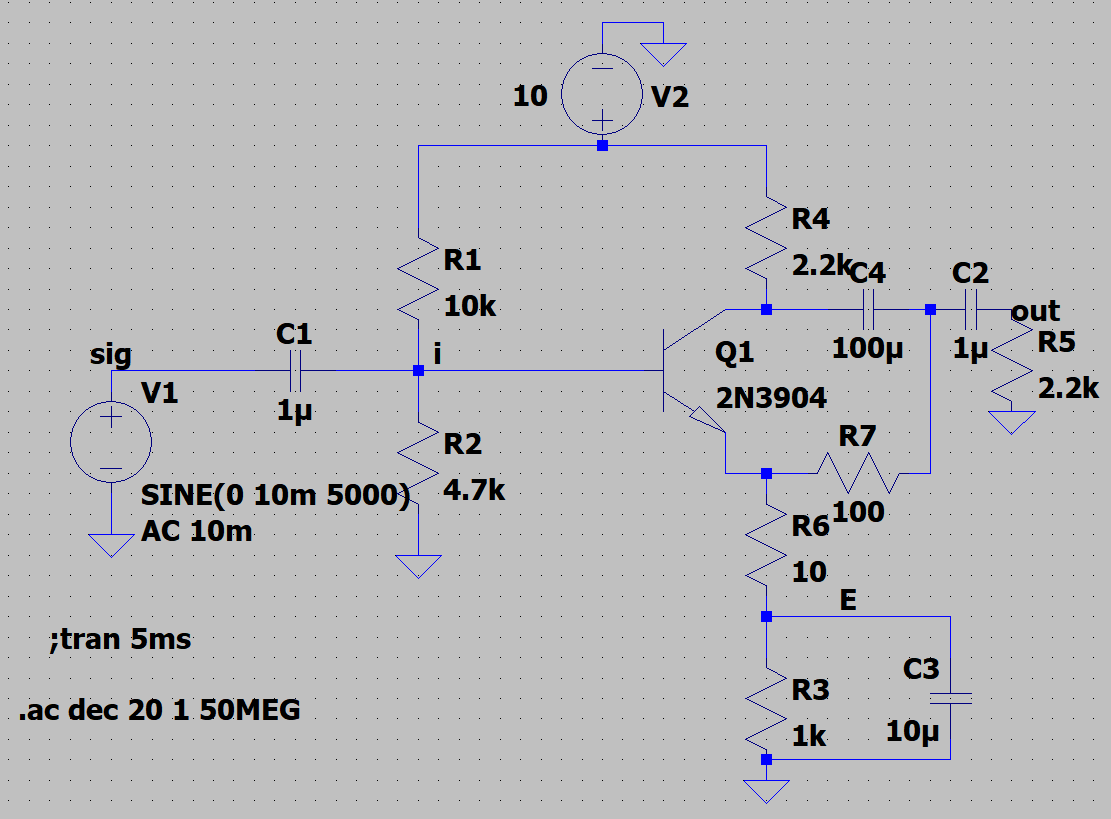
\includegraphics[width=\columnwidth]{circuito-simulacao.PNG}
    		\caption{Circuito simulado no \textit{Software} LT{\ssmall SPICE} XVII.}
    		\label{circuito ltspice}
    		\end{center}
    	\end{figure}
    	
    \tab Em seguida, verificou-se o ganho A\textsubscript{f} do circuito. Esse dado é observado na Figura \ref{ganho af simulação}
    	
    	\begin{figure}[H]
    		\begin{center}
    		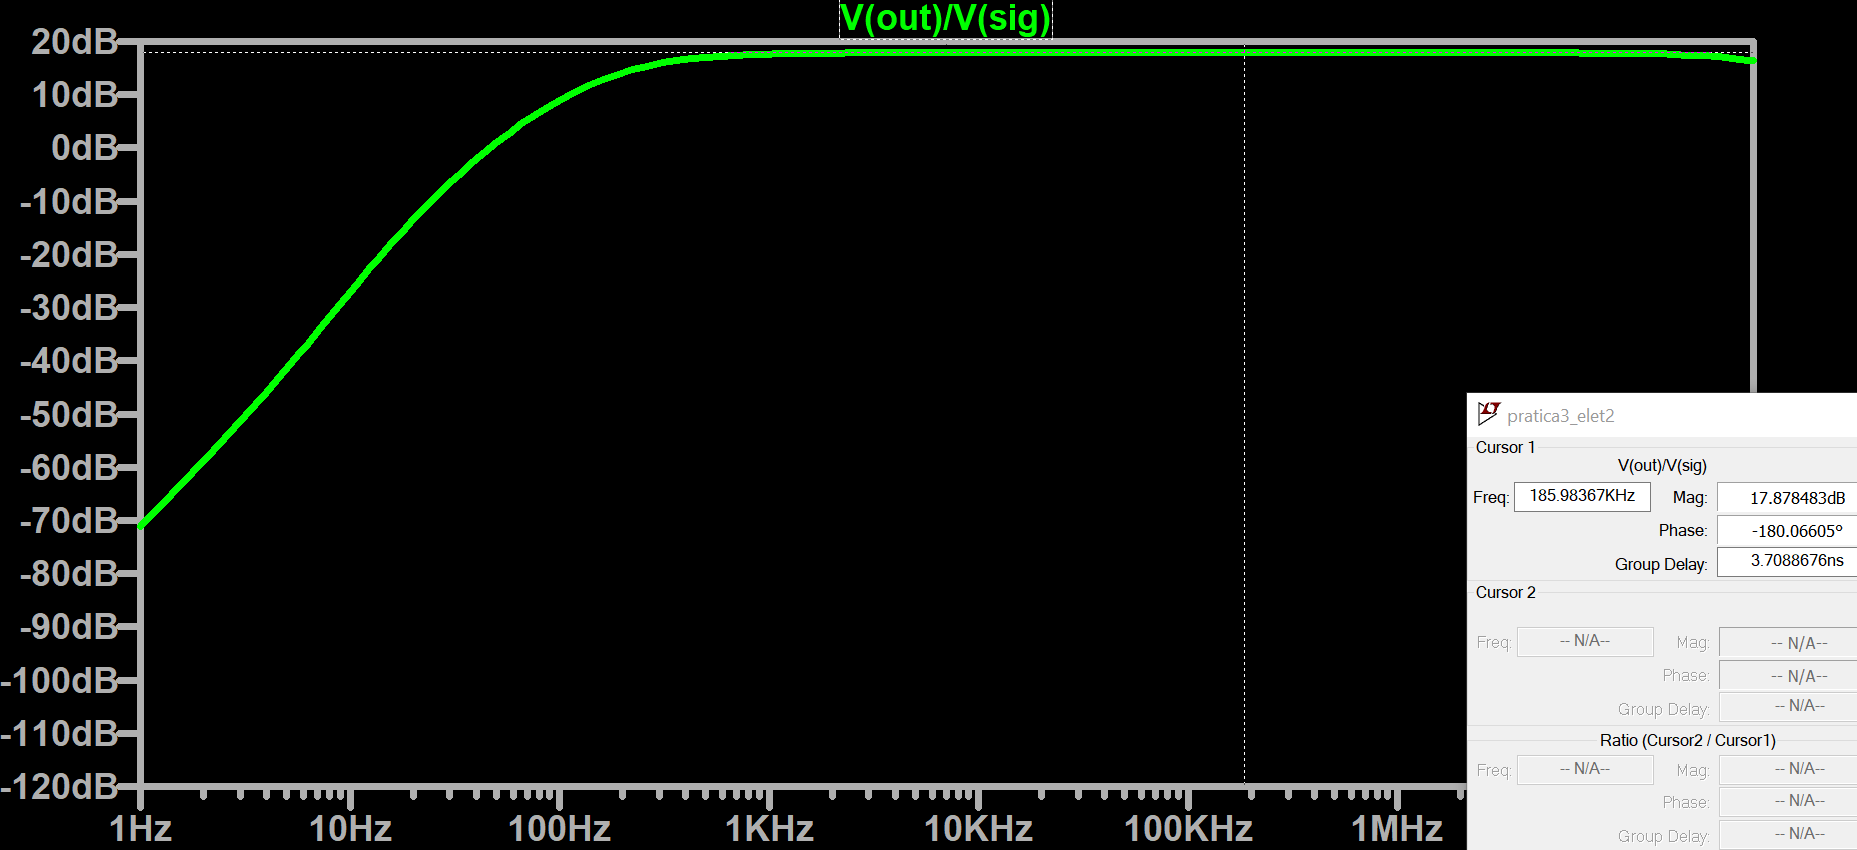
\includegraphics[width=\columnwidth]{ganhoAf-novo.PNG}
    		\caption{Forma de onda do ganho A\textsubscript{f}.}
    		\label{ganho af simulação}
    		\end{center}
    	\end{figure}
    	
    \tab Nota-se que o ganho simulado de 17,87 dB é consistente com o ganho calculado.
    
\section{Equipamentos Utilizados}

    \tab Durante a prática, os seguintes instrumentos foram utilizados para a montagem e avaliação do circuito:
     \begin{itemize}
        \item Multímetro digital.
        
        \item Osciloscópio com gerador de sinais.
        
        \item Fonte de alimentação contínua.
        
        \item \textit{Protoboard}.
        
        \item Um transistore NPN.
        
        \item Resistores de $10 \: k\Omega,\: 4,7 \: k\Omega,\: 2,2 \: k\Omega$, $1 \: k\Omega$, $100 \: \Omega$ e $10 \: \Omega$.
        
        \item Capacitores de $1 \: \mu F,\: 10 \: \mu F$ e $100 \: \mu F$.
        
     \end{itemize}
        
        
\section{Procedimento Experimental}

    \tab O circuito sugerido foi montado com os respectivos componentes comprados pela equipe e o osciloscópio foi usado para determinar o ganho de tensão ao qual o sinal foi submetido.
    
    
        
        \begin{figure}[H]
    		\begin{center}
    		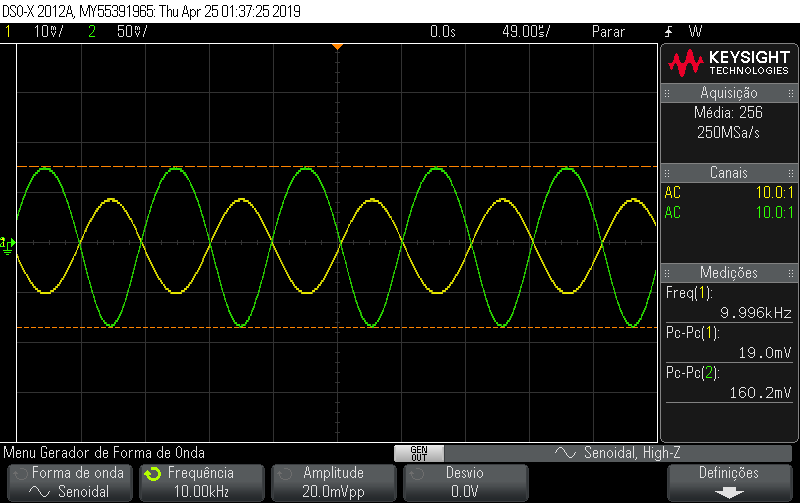
\includegraphics[width=\columnwidth]{ganhoAf-pratica.png}
    		\caption{Ganho A\textsubscript{f} Observado no Osciloscópio.}
    		\label{ganho af pratica}
    		\end{center}
    	\end{figure}
    	
    \tab Observa-se que o ganho encontrado experimentalmente é 18,51 dB e está consistente com o ganho calculado e simulado.
        
    \tab Em seguida utilizou-se dois potenciômetros em momentos distintos para medir as resistências vistas pelos terminais. Coloca-se o potenciômetro no terminal desejado e varia-se a resistência até que o ganho A\textsubscript{f} seja reduzido à metade. Utiliza-se um potenciômetro em paralelo com $R_2$ para medir R\textsubscript{if} e outro em paralelo com R\textsubscript{L} para medir R\textsubscript{of}. Os valores obtidos de R\textsubscript{if} e R\textsubscript{of} foram $3,98 \: k\Omega$ e $170 \: \Omega$ respectivamente.
    
    
\section{Análise dos Resultados}

    \tab  Como demonstrado anteriormente, o ganho encontrado experimentalmente foi de 18,51 dB, enquanto o ganho encontrado na fase de cálculos foi de 18,38 dB. Isso mostra que a porcentagem de discrepância (erro) é de, aproximadamente, 0,7\%. Conclui-se, portanto, que o erro associado ao ganho do amplificador transistorizado é irrelevante. O grupo comparou os valores experimental e teórico de R\textsubscript{if}. Notou-se que estes valores foram muito distantes e, portanto, determinou-se que a medida prática deve ter sido contaminada por algum erro humano. Quanto à medida do resistor R\textsubscript{of}, houve uma discrepância de, aproximadamente, 43\%. Esta distância, é claro, deveria ser menor. Porém, o efeito indesejado deve ter sido provocado pelo capacitor CA, já que o grupo tentou resolver este impasse durante o experimento, mas foi malsucedido.  Observa-se, também, na seção teórica, que, para garantir maior estabilidade ao sistema, sacrificou-se uma parcela notável do ganho original. Assim, o modelo usado na teoria se mostrou válido quando o grupo realizou certas considerações críticas a respeito do experimento. Por último, observou-se que, apesar de maior estabilidade, o sistema possui menor ganho e, portanto, a escolha por este circuito depende das necessidades do projetista.

\end{document}